\subsection{Гироскоп. Прецессия гироскопа}

\begin{definition}
    Гироскопом называется массивное аксиально-симметричное 
твердое тело, способное вращаться вокруг оси симметрии с
большой угловой скоростью. Ось симметрии гироскопа
называют собственной осью гироскопа или просто осью
гироскопа. Она может менять свое положение в пространстве.
\end{definition}

\begin{example}
    Юла, маховики гироскопических
компасов, роторы турбин различного назначения и пр.
\end{example}

\begin{definition}
    Движение гироскопа с необходимостью представляет собой
движение твердого тела с одной неподвижной точкой,
которая называется точкой опоры гироскопа.
В случае, если неподвижная точка отсутствует, быстро
вращающееся аксиально-симметричное тело называют
волчком.
\end{definition}

\begin{definition}
    Уравновешенным или ненагруженным называется гироскоп, ось 
вращения которого вертикальна и момент М всех внешних сил 
относительно неподвижной точки гироскопа равен нулю: М=0.
\end{definition}

\begin{wrapfigure}{l}{0.22\linewidth}
    \centering
    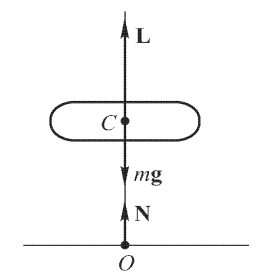
\includegraphics[width=\linewidth]{imgs/q12i1.png}
\end{wrapfigure}

В этом случае поведение гироскопа 
совпадает со свободным вращением вокруг 
оси симметрии – центральной главной оси:
$$L(t)=L(0)$$
Ось гироскопа все время сохраняет свое 
направление.

Если ось гироскопа находится в вертикальном положении, 
то гироскоп может вращаться в этом положении довольно долго.

\ 

\ 

\ 

\ 

\ 


\begin{definition}
    Прецессия нагруженного гироскопа

    Если ось быстро вращающегося гироскопа слегка отклонить от вертикали, то она
    начнет прецессировать вокруг вертикального положения, т.е. совершать
    вращательное движение по поверхности конуса.
\end{definition}

\begin{wrapfigure}{r}{0.3\linewidth}
    \centering
    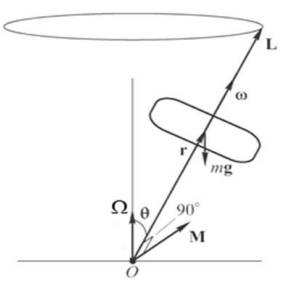
\includegraphics[width=\linewidth]{imgs/q12i2.png}
\end{wrapfigure}

    Прецессию гироскопа можно
представить как суперпозицию вращений
вокруг двух осей: быстрого вращение
вокруг собственной оси и относительно
медленного вращения вокруг вертикали.
Пересечение этих осей вращения дает
неподвижную точку гироскопа.
Угловая скорость $\omega$ вращения вокруг
собственной оси называется
собственной угловой скоростью
гироскопа.

Угловая скорость $\Omega$ вращения вокруг вертикальной оси называется угловой 
скоростью прецессии гироскопа:  $\Omega << \omega$

Чем больше собственная частота вращения тем меньше частота прецессии $\Omega \sim 1/\omega$

\ 

\ 

\ 

\ 

\ 

Приближенная теория гироскопа

$$\frac{dL}{dt} = M$$


\begin{wrapfigure}{l}{0.2\linewidth}
    \centering
    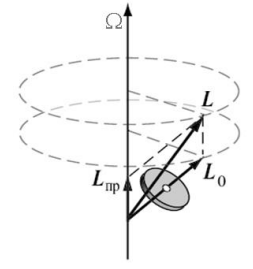
\includegraphics[width=\linewidth]{imgs/q12i3.png}
\end{wrapfigure}

В приближенной теории полагается, что вектор момента импульса L гироскопа все 
время ориентирован вдоль оси гироскопа и равен моменту импульса собственного 
вращения: $L \cong L_0 = I\omega$

$I$ - момент инерции гироскопа относительно своей оси: $I = I_{||}$

Если скорость прецессии много ниже 
собственной скорости вращения $\Omega << \omega$, то отклонение вектора $L$ от оси гироскопа 
незначительно, и им можно пренебречь. 


\ 

\ 

\ 

\ 

\ 

\

Ось гироскопа отклонена от вертикали 
на угол $\Theta$

Момент внешних сил относительно
неподвижной точки создает только сила
тяжести гироскопа, приложенная к его
центру масс, расположенному на оси
гироскопа и удаленному от его
неподвижной тоски на расстояние $r$

$$M = r \times mg$$

$r$ - радиус вектор, проведенный из неподвижной точки O в центр масс 
гироскопа

\begin{figure}[h]
    \centering
    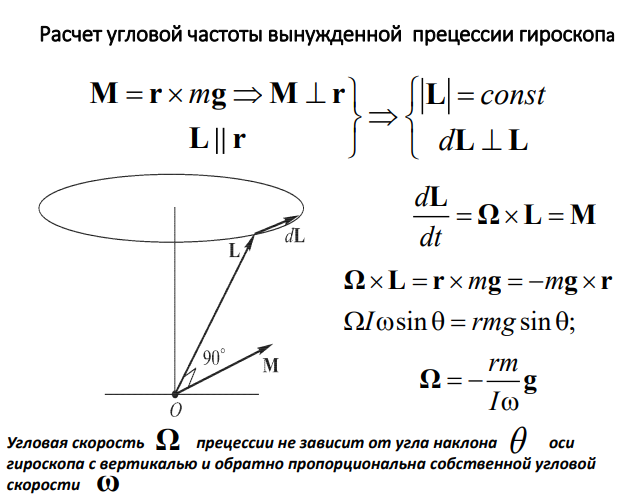
\includegraphics[width=0.4\linewidth]{imgs/q12i4.png}
\end{figure}
\begin{figure}[h]
    \centering
    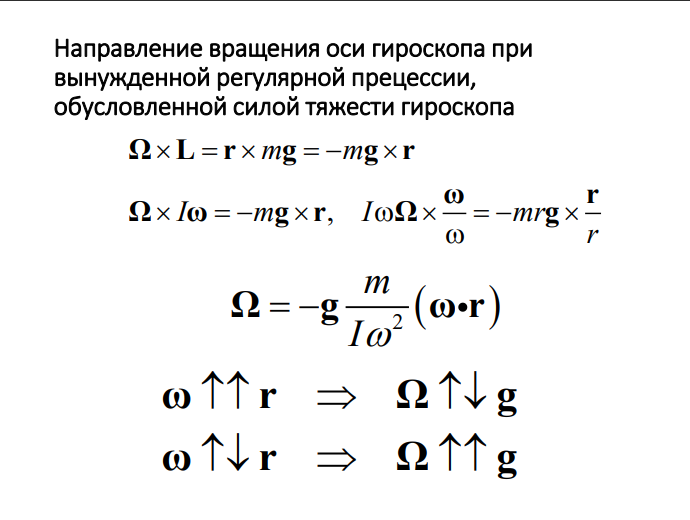
\includegraphics[width=0.42\linewidth]{imgs/q12i5.png}
\end{figure}
\begin{figure}[h]
    \centering
    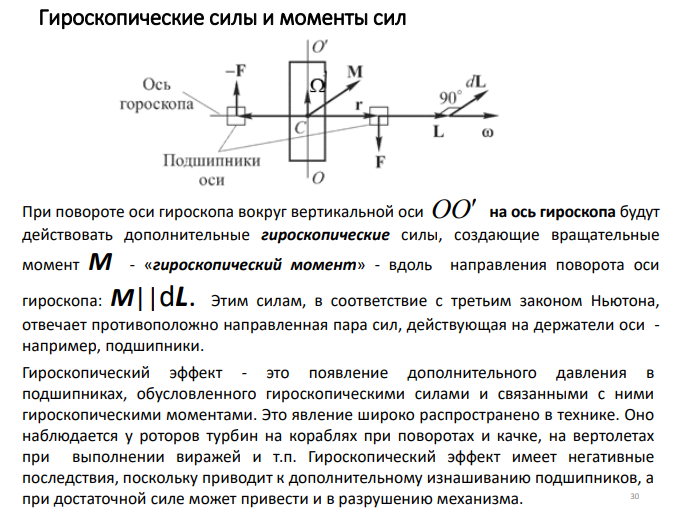
\includegraphics[width=0.5\linewidth]{imgs/q12i6.png}
\end{figure}
\begin{figure}[h]
    \centering
    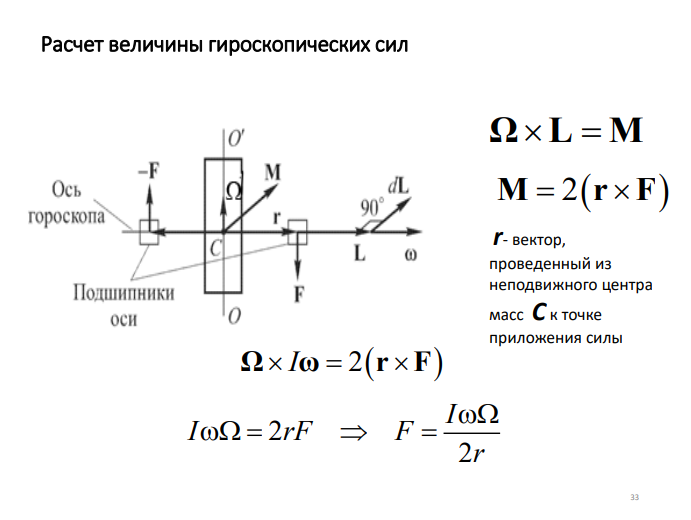
\includegraphics[width=0.5\linewidth]{imgs/q12i7.png}
\end{figure}

